\documentclass[11pt]{article}
%----------------------------------------------------------------------------------------------
%   PACKAGES AND CONFIGURATIONS 
%----------------------------------------------------------------------------------------------

\usepackage{lastpage}
\usepackage{hyperref}
\usepackage{graphicx}
\usepackage{pgfplots}
\pgfplotsset{compat=1.17}
\usepackage{xcolor}
\usepackage{amsmath}
\usepackage{bussproofs}
\usepackage{amssymb}
\usepackage{amsfonts}
\usepackage{graphicx}
\usepackage{booktabs}
\usepackage{listing}
\usepackage{etoolbox}
\usepackage{latexsym}
\usepackage{listings}
\usepackage[utf8]{inputenc}
\usepackage{caption}
\graphicspath{{./img}}

\DeclareCaptionFont{white}{\color{white}}
\DeclareCaptionFormat{listing}{%
  \parbox{\textwidth}{\colorbox{gray}{\parbox{\textwidth}{#1#2#3}}\vskip-4pt}}
\captionsetup[lstlisting]{format=listing,labelfont=white,textfont=white}
\lstset{frame=lrb,xleftmargin=\fboxsep,xrightmargin=-\fboxsep}

%-----------------------------------------------------------------------------------------------
%   MARGINS
%-----------------------------------------------------------------------------------------------

\usepackage{geometry}
\geometry{
    paper=a4paper,
    top=3cm,
    bottom=3cm,
    left=2.5cm,
    right=2.5cm,
    headheight=14pt,
    footskip=1.4cm,
    headsep=1.2cm,
}

%-----------------------------------------------------------------------------------------------
%   FONT
%-----------------------------------------------------------------------------------------------

\usepackage[utf8]{inputenc}
\usepackage[T1]{fontenc}

\usepackage[sfdefault,light]{roboto}

%-----------------------------------------------------------------------------------------------
%   HEADER AND FOOTER   
%-----------------------------------------------------------------------------------------------

\usepackage{fancyhdr}
\pagestyle{fancy}

\lhead{\small\classHomework\ifdef{\className}{\ (\className):}{}\ \homeworkTitle}
\chead{}
\rhead{\small\ifdef{\authorName}{\authorName}{\ifdef{dueDate}{Due\ \dueDate}{}}}

\lfoot{}
\cfoot{\small Page\ \thepage\ of\ \pageref{LastPage}}
\rfoot{
\includegraphics[scale=0.06]{logo-unige.png}}

\renewcommand\headrulewidth{0.5pt}

%-------------------------------------------------------------------------------------------------
%   TITLE PAGE
%-------------------------------------------------------------------------------------------------

\author{\textbf{\authorName}}
\date{}

\title{
    \thispagestyle{empty}
    \vspace{0.2\textheight}
    \textbf{\classHomework:\ \homeworkTitle}\\[-4pt]
    \ifdef{\classHomework}{{\small Due\ on\ \dueDate}\\}{}
    \ifdef{\className}{{\large \textit{\className}}}{}
    \vspace{0.32\textheight}

    
\includegraphics[scale=0.2]{logo-unige.png}
}


\begin{document}
    
    \maketitle
    \thispagestyle{empty}
    \newpage

    \tableofcontents
    
    \newpage

\hypertarget{introduction}{%
\section{Introduction}\label{introduction}}

This report delves into the parallel computation of the Mandelbrot set
using OpenMP, with a focus on comparing static and dynamic scheduling.
The Mandelbrot set, a complex fractal, presents a significant
computational challenge, making it an ideal candidate for parallel
processing. This study aims to assess the performance implications of
different scheduling strategies in OpenMP, highlighting how they affect
computation efficiency in a parallelized environment.

\hypertarget{methodology}{%
\section{Methodology}\label{methodology}}

The Mandelbrot set generation code from TP 5 was adapted for this
experiment, using two separate implementations to facilitate static and
dynamic scheduling. This bifurcation allowed each version to be
specifically optimized through compilation, a crucial factor in parallel
computing performance. Static scheduling was implemented by dividing the
workload into predetermined chunks, while dynamic scheduling was applied
to allocate workload in smaller, adaptable chunks based on thread
availability.

\hypertarget{results-and-analysis}{%
\section{Results and Analysis}\label{results-and-analysis}}

\hypertarget{execution-time-comparison}{%
\subsection{Execution Time
Comparison}\label{execution-time-comparison}}

The experiment involved recording execution times for both static and
dynamic scheduling across varying numbers of threads (1, 2, 4, 8, 16,
32, 64, 128, and 256). The results are visualized in the graph below:

\begin{figure}[ht]
\centering
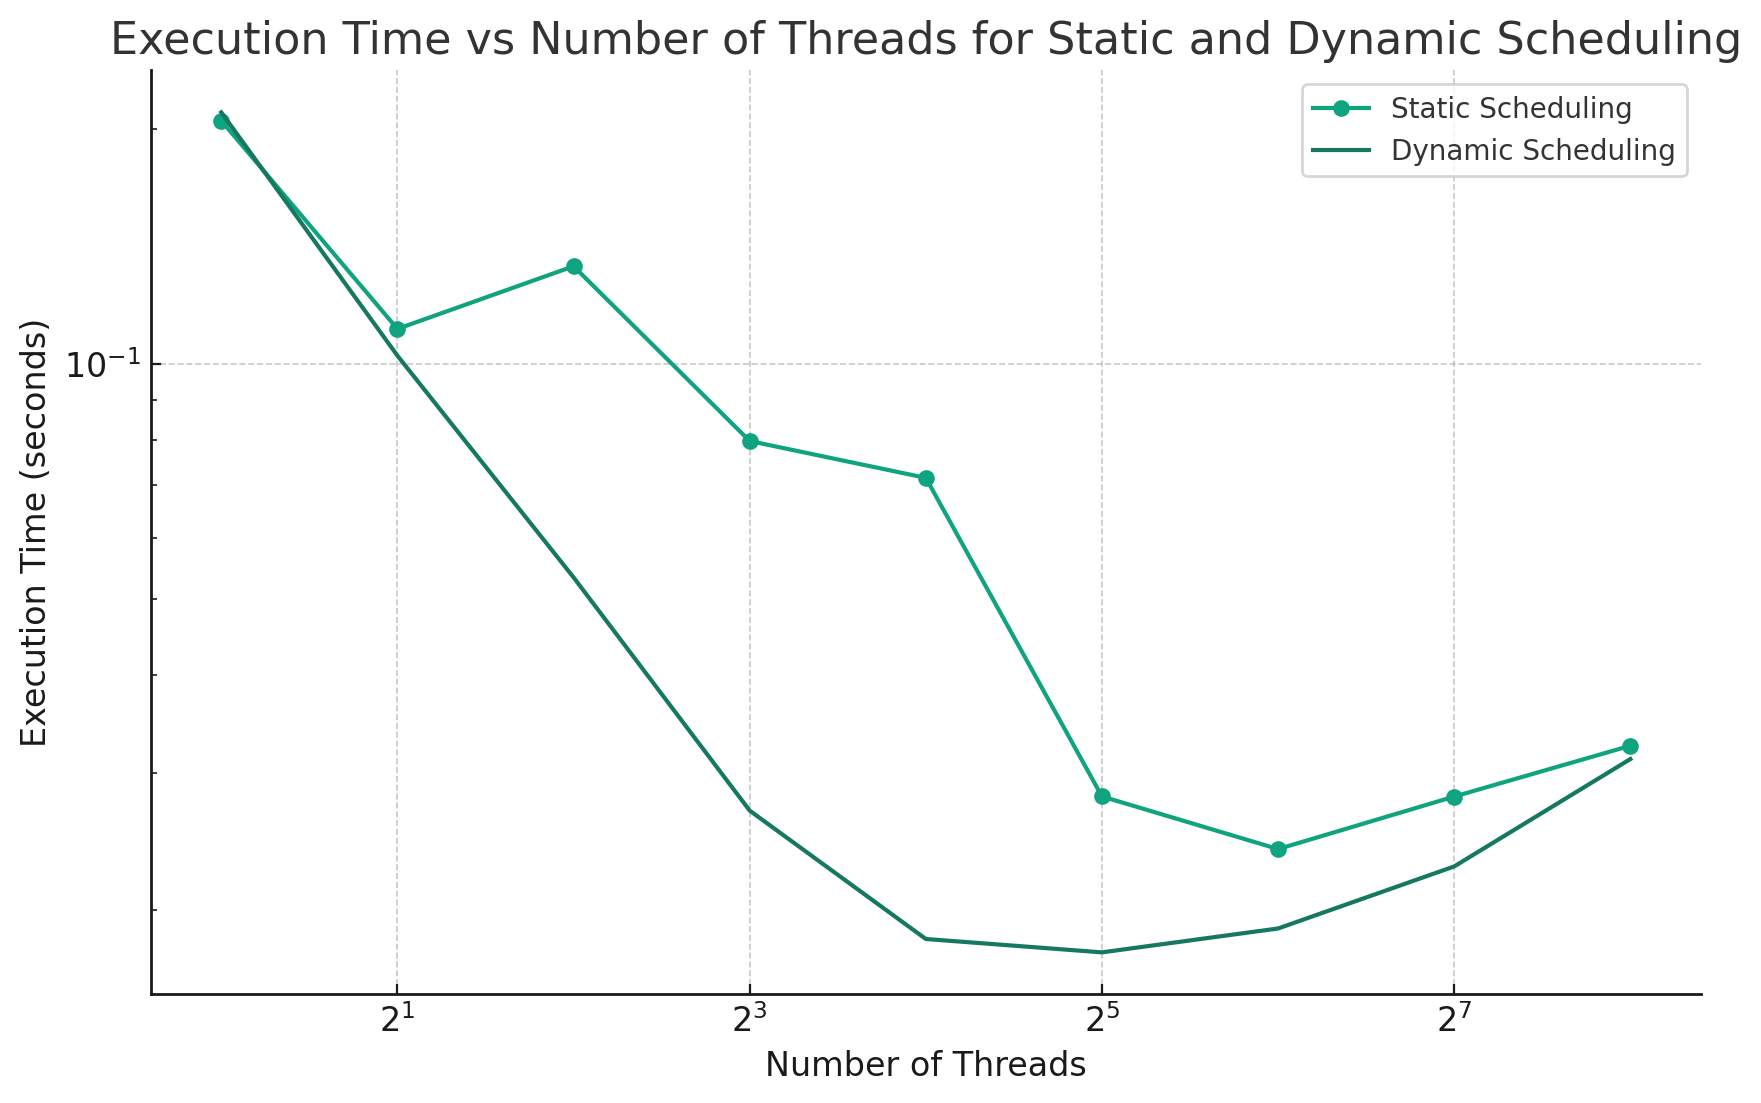
\includegraphics[width=0.8\textwidth]{./img/results.png}
\caption{Execution Time vs Number of Threads for Static and Dynamic
Scheduling}
\end{figure}

Key observations from the graph include: - Both scheduling strategies
show decreased execution time with an increase in the number of threads,
affirming the advantage of parallel processing. - Dynamic scheduling
consistently outperforms static scheduling, especially at higher thread
counts, indicating superior load balancing and adaptability. - The
scaling of performance gains is non-linear, with both strategies showing
diminishing returns or slight increases in execution times at higher
thread counts.

\hypertarget{performance-variations}{%
\subsection{Performance Variations}\label{performance-variations}}

Static scheduling exhibits an increase in execution time beyond 64
threads. In contrast, dynamic scheduling maintains relatively stable
times after an initial drop, suggesting its efficiency in managing high
thread numbers.

\hypertarget{challenges}{%
\section{Challenges}\label{challenges}}

One of the main challenges was optimizing load balancing to maximize
performance. Static scheduling, although simpler, often led to uneven
workload distribution. In contrast, dynamic scheduling provided better
load balancing, adapting to runtime conditions but was more complex to
implement. The separate compilations for each scheduling strategy
highlight the importance of compilation in parallel computing, where
optimization can significantly impact performance.

\hypertarget{running-the-code}{%
\section{Running the Code}\label{running-the-code}}

The code can be compiled using the provided \texttt{Makefile} by running
\texttt{make} in the terminal. The executable can then be run using
\texttt{./fractal\_static} or \texttt{./fractal\_dynamic} for static and
dynamic scheduling, respectively. The number of threads can be specified
using the \texttt{-t\ \textless{}num\_threads\textgreater{}} flag.

\hypertarget{conclusion}{%
\section{Conclusion}\label{conclusion}}

This study highlights the importance of selecting an appropriate
scheduling strategy in parallel computing. Dynamic scheduling, while
more complex, offers superior performance and load balancing, especially
at higher thread counts. This experiment contributes valuable insights
into optimizing parallel computing tasks, demonstrating how different
scheduling strategies can significantly influence performance in the
context of OpenMP and the Mandelbrot set computation.

\end{document}